%%%%%%   TIPO DE DOCUMENTO: Artículo   %%%%%%
\documentclass[letterpaper,11pt,twoside]{report}

\usepackage[spanish]{babel} %Idioma
\usepackage{graphicx} %Imágenes
\usepackage[utf8]{inputenc} %Acentos
\usepackage{hyperref} %Links
\usepackage{xspace}

\usepackage{listings}
\usepackage{verbatim}
\usepackage{amsmath, amssymb}
\usepackage{amsmath}
\usepackage[active]{srcltx}
\usepackage{amssymb}
\usepackage{amscd}
\usepackage{makeidx}
\usepackage{amsthm}
\usepackage{algpseudocode}
\usepackage{algorithm}
\usepackage{float}
\usepackage{caption}

\renewcommand{\baselinestretch}{1}
\renewcommand{\thesection}{\Roman{section}} 
\renewcommand{\thesubsection}{\thesection.\Roman{subsection}}

\setcounter{page}{1}
\setlength{\textheight}{21.6cm}
\setlength{\textwidth}{14cm}
\setlength{\oddsidemargin}{1cm}
\setlength{\evensidemargin}{1cm}
\pagestyle{myheadings}
\captionsetup[figure]{position=below, skip=0pt}
\thispagestyle{empty}
\markboth{\small{Servicio Social, Jorge Mart\'inez.}}{\small{.}}
\date{}

\begin{document}
	\centerline{\bf REPORTE FINAL, \today}
	\centerline{}
	\begin{center}
		\Large{\textsc{}}
	\end{center}
	
	\centerline{}
	\centerline{\textbf{Martínez Buenrostro Jorge Rafael}}
	\centerline{}
	
	\centerline{$correo, molap96@gmail.com$}
	
        \centerline{Universidad Aut\'onoma Metropolitana} 
	\centerline{Unidad Iztapalapa, M\'exico}
	
	\bigskip


	%  1. Datos Generales
	\section{Datos generales y matrícula del prestador}
	\begin{description}
		\item[Nombre] - Jorge Rafael Mart\'inez Buenrostro
		\item[Matr\'icula] - 2203040824
		\item[Carrera] - Licenciatura en Computación
	\end{description}


	%  2. Lugar y periodo de realización
	\section{Lugar y periodo de realizaci\'on}
	\begin{description}
		\item[] Universidad Aut\'onoma Metropolitana Unidad Iztapalapa
		\item[] Departamento de Ingenier\'ia El\'ectrica
		\item[] \'Area de Computaci\'on y Sistemas
		\item[] Laboratorio T-169
	\end{description}
	\noindent El proyecto se llevar\'a a cabo del \textbf{15 de Abril de 2025 al 15 de Noviembre de 2025}. Estar\'a dividido en las etapas
	que se listan en la siguiente tabla, cada una con la duraci\'on indicada.
	\begin{figure}[H]
		\centering
		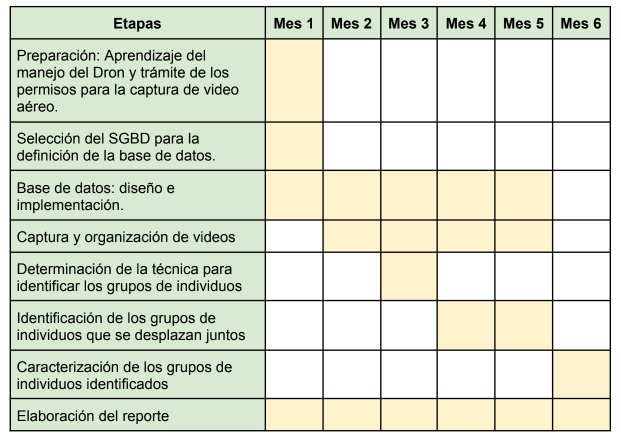
\includegraphics[width=0.6\textwidth]{img/gantt.png}
	\end{figure}


	%  3. Unidad, División y licenciatura que hay cursado
	\section{Unidad, Divisi\'on y licenciatura cursada}
	\begin{description}
		\item[Unidad] - Iztapalapa
		\item[Divisi\'on] - Ciencias B\'asicas e Ingenier\'ia
		\item[Licenciatura] - Computaci\'on   
	\end{description}


	%  4. Nombre del programa y/o proyecto en el que se participo
	\section{Nombre del proyecto}
	\noindent Construcci\'on de una base de datos de videos a\'ereos y su an\'alisis v\'ia herramientas de IA

	%  5. Nombre y cargo del asesor
	\section{Nombre y cargo del asesor}
	\begin{description}
		\item[Nombre] - Dra. Elizabeth P\'erez Cort\'es
		\item[Cargo] - Profesor Investigador Titular "C" TC TI
	\end{description}

	%  6. Participantes 
	\section{Participantes}
	\noindent Jorge Rafael Mart\'inez Buenrostro

	%  7. Introduccion
	\section{Introducci\'on}


	%  8. Objetivos generales y específicos
	\section{Objetivos generales y espec\'ificos}
	

	%  9. Metodologia utilizada
	\section{Metodolog\'ia utilizada}

	%  10. Actividades realizadas
	\section{Actividades realizadas}

	%  11. Objetivos y metas alcanzados
	\section{Objetivos y metas alcanzados}

	%  12. Resultados y conclusiones
	\section{Resultados y conclusiones}

	%  13. Recomendaciones
	\section{Recomendaciones}

	%  14. Bibliografia
	\section{Bibliograf\'ia}
\end{document}

